\section{Born from Data}

The exponential increase in data generation has profoundly transformed the digital information landscape, with the total volume of data created, captured, copied, and consumed globally reaching approximately 120 zettabytes in 2023. This number will rise to 147 zettabytes by the end of 2024 with expectations to surpass 181 zettabytes by 2025 \cite{taylor2023volume}. This rapid expansion of the data ecosystem has catalyzed significant advancements in artificial intelligence (AI), particularly in the development of large language models (LLMs) \cite{zhao2023survey}. LLMs, known for their exceptional ability to comprehend, generate, and manipulate human language, have become a cornerstone in the evolution of AI chatbots \cite{brown2020language}.

\begin{figure}[h!]
    \centering
    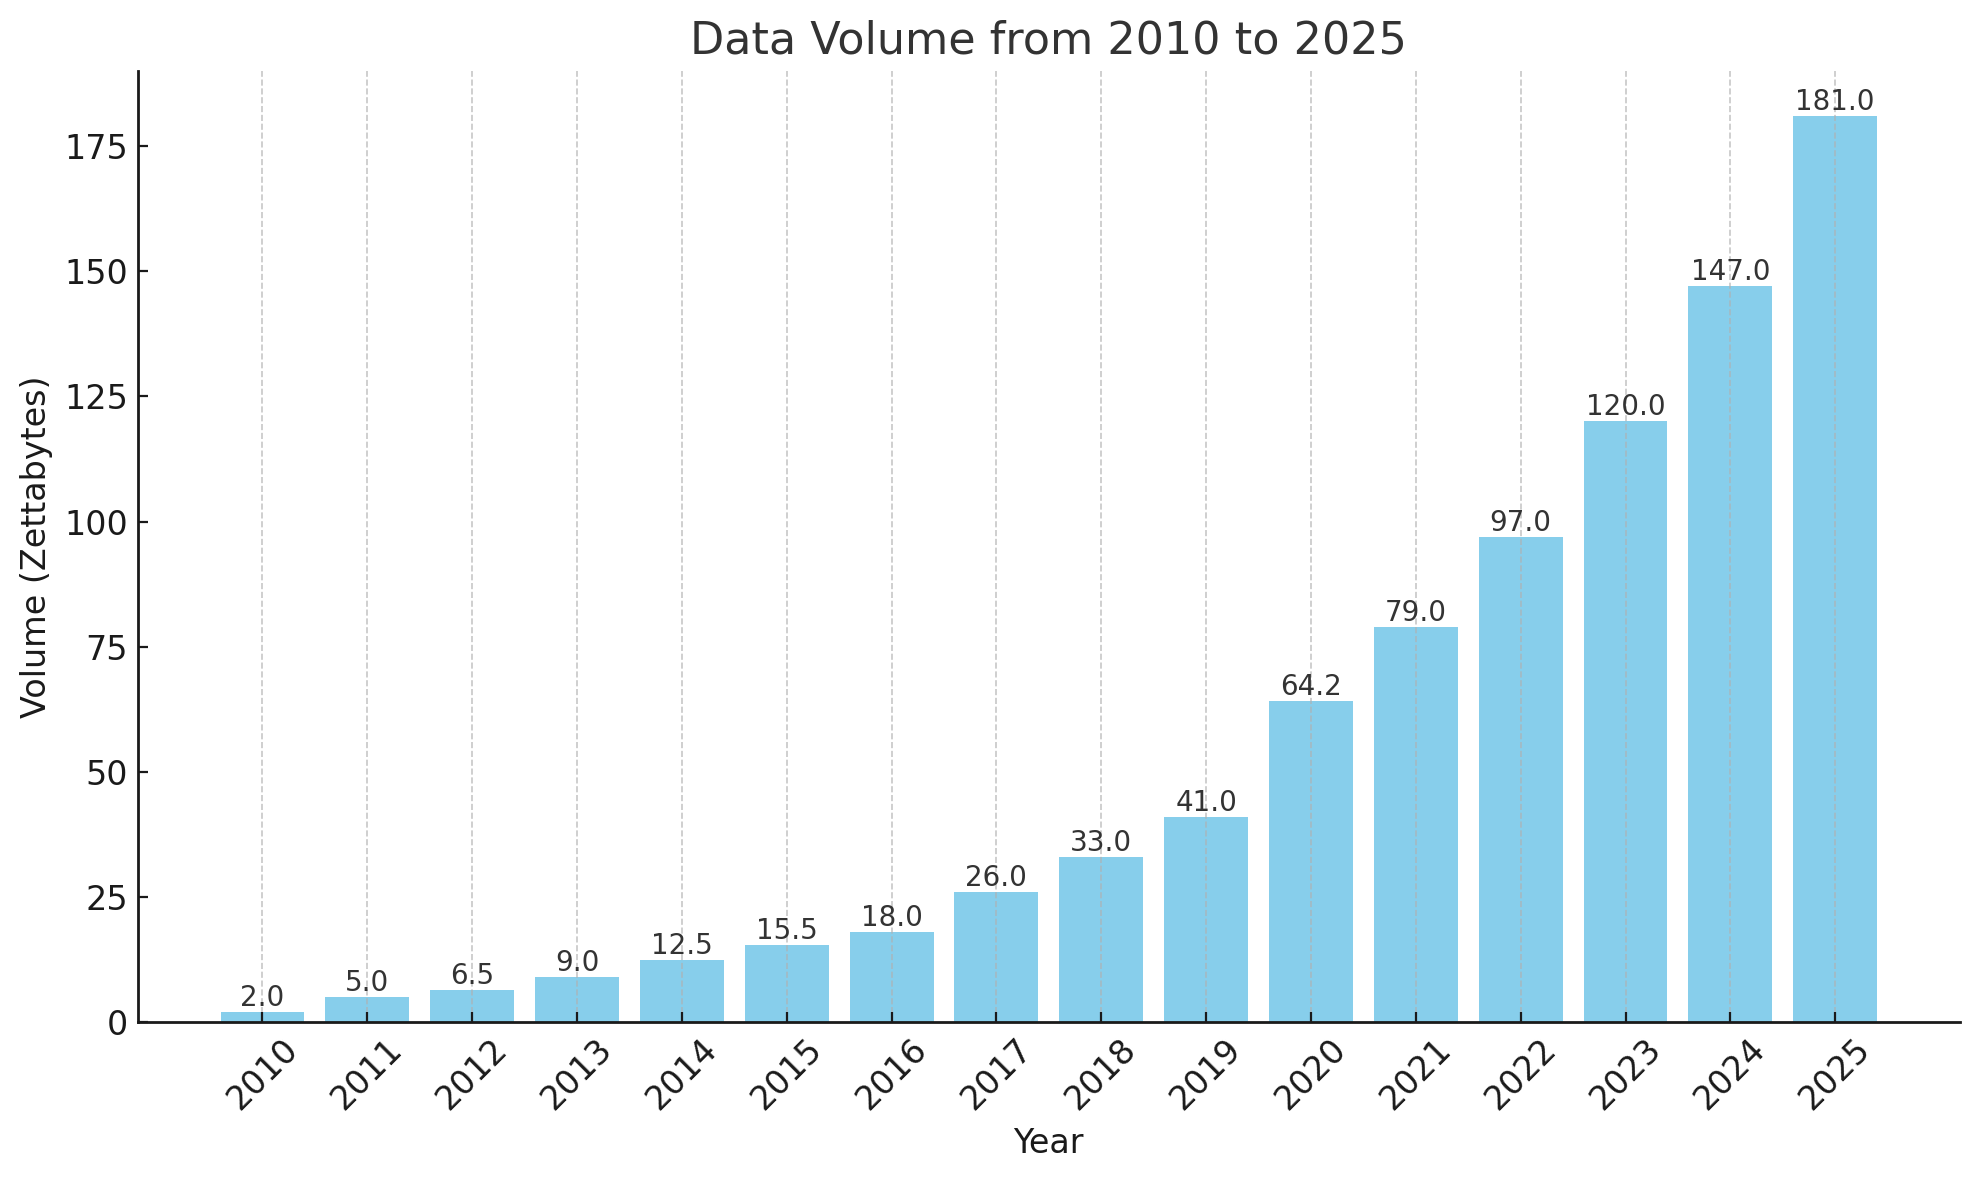
\includegraphics[width=0.8\textwidth]{images/literature/data-viz.png}
    \caption{Data Volume from 2010 to 2025. \textit{Source:} \cite{taylor2023volume}}
    \label{fig:data_volume}
\end{figure}

In the era of AI-driven chatbots, LLMs have emerged as pivotal tools, powering conversational capabilities and enabling human-like interactions \cite{koubaa2023exploring}. The surge in data, coupled with advancements in computational techniques, has significantly enhanced the functionality of LLM-based chatbots, making them valuable across various sectors. These chatbots' ability to understand and respond with unprecedented contextual relevance and accuracy, while managing vast streams of information, has rendered them crucial in domains such as education, research, healthcare, and many others \cite{dam2024complete}.

\begin{figure}[h!]
    \centering
    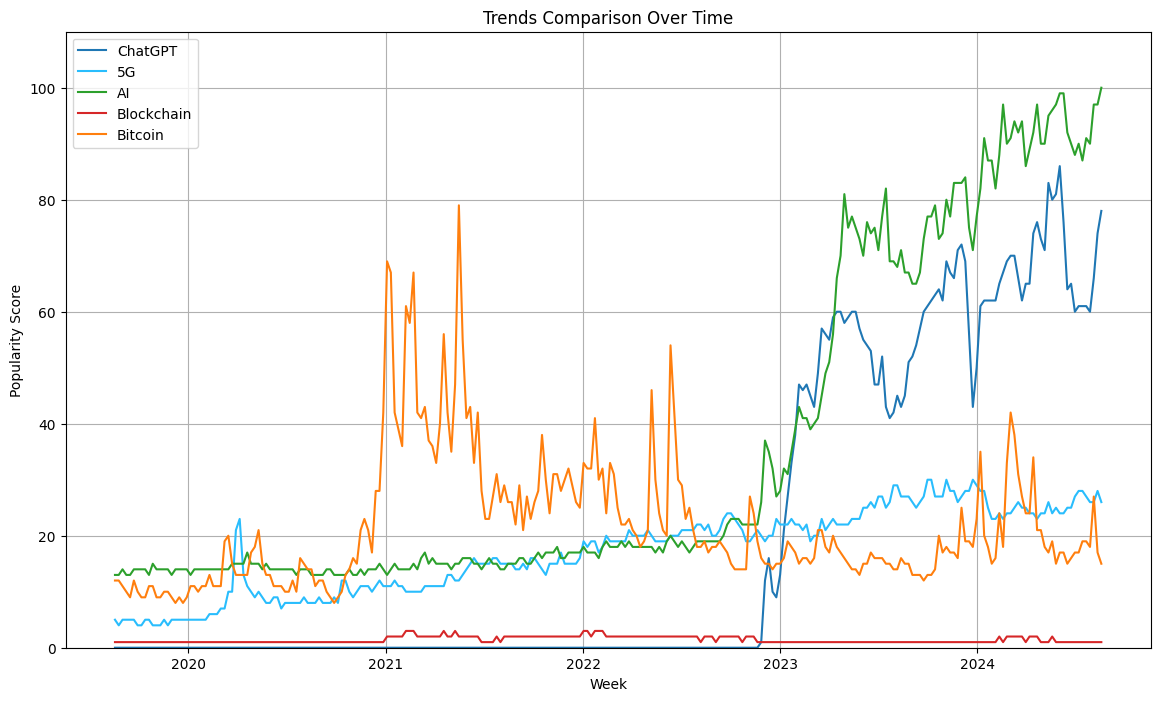
\includegraphics[width=0.9\textwidth]{images/literature/trends-comparison.png}
    \caption{Trends Comparison Over Time: The graph compares the popularity scores of ChatGPT, AI, 5G, Bitcoin, and Blockchain technologies over the period from 2020 to 2024. \textit{Source:} \cite{googletrends2023}}
    \label{fig:chatgpt_popularity}
\end{figure}

In March 2023, OpenAI launched GPT-4, building on the widespread success of ChatGPT 3.5, which was released in November 2022 \cite{bahrini2023chatgpt, zhang2023one}. The exponential rise in popularity of ChatGPT and AI, as depicted in Figure \ref{fig:chatgpt_popularity}, underscores its dominance over other emerging technologies such as 5G, Bitcoin, and Blockchain \cite{googletrends2023}. In response to this surge, Google launched BARD in early 2023, later rebranded as Gemini, its first LLM-based chatbot, thereby significantly enriching the expanding ecosystem of LLM-powered conversational agents \cite{wikipedia2024gemini}. Moreover, a multitude of other LLM-based chatbots are currently under development, further advancing this dynamic field.

Given the vast potential and expanding use of AI chatbots, there is a critical need for thorough research and evaluation to optimize their performance. As the field rapidly evolves, an overwhelming volume of research demands comprehensive analysis. This chapter provides a review of LLM-based chatbots, beginning with their evolution from early AI chatbots to the current era dominated by LLMs. It examines key applications across sectors and explores the importance of personalization in enhancing user experience. This review offers insights for improving the effectiveness and reliability of AI chatbots.

\section{The Evolution of Chatbots}

This section examines the evolution of chatbots, tracing their development from the advent of early conversational systems to the present-day advancements in LLM-powered chatbots. It provides an overview of the significant milestones in chatbot technology, culminating in the transformative impact of Large Language Models (LLMs). An overview of the history and evolution of LLMs, which have played a pivotal role in this transformation, will be explored in the dedicated Chapter 3. Figure \ref{fig:chatbot_venn_diagram} provides a visual representation of the interrelationship between pre-LLMs chatbots, the development of LLMs, and the emergence of LLM-based chatbots. The intersection in the diagram represents the point at which early chatbot technology and LLM advancements converge, marking the advent of a new era of highly capable and contextually aware chatbots.

\begin{figure}[h!]
    \centering
    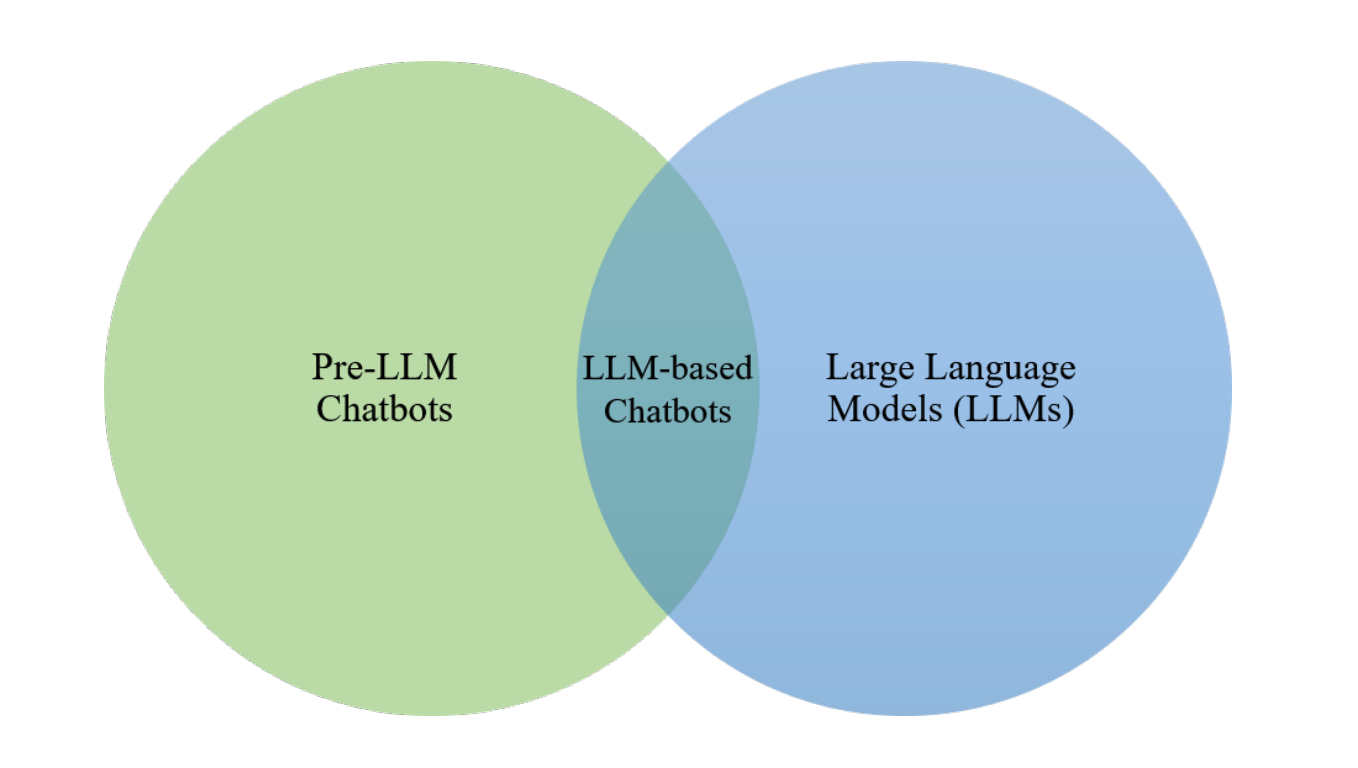
\includegraphics[width=0.7\textwidth]{images/literature/venn_diagram.png}
    \caption{Pre-LLMs chatbots meet LLMs. \textit{Source:} \cite{dam2024complete}}
    \label{fig:chatbot_venn_diagram}
\end{figure}

\subsection{Pre-LLMs Era of Chatbots}

The origins of chatbots trace back to the pivotal question posed by Alan Turing in 1950: "Can machines think?". This query laid the groundwork for what is now recognized as the Turing Test, where a human participant engages in a text-based interaction with an unseen entity, attempting to discern whether they are conversing with a machine or another human \cite{turing2009computing}. This concept catalyzed the early development of chatbots, which, while rudimentary by contemporary standards, marked significant strides in artificial intelligence during their time.

\subsubsection{1960–1980: Foundational Developments}

Between 1960 and 1980, the first wave of chatbots emerged, setting the stage for future advancements. One of the earliest examples is ELIZA, developed in 1966 at MIT. ELIZA was designed to simulate a Rogerian psychotherapist by identifying keywords and applying pattern matching techniques, although it lacked genuine comprehension of the inputs \cite{weizenbaum1966eliza}. Despite its limitations, ELIZA garnered significant attention for its ability to mimic human-like interactions, even forming emotional connections with users, which later sparked ethical debates \cite{zimmerman2023human}. Another notable chatbot from this era is PARRY, introduced in 1972 to emulate a person with paranoid schizophrenia. PARRY advanced chatbot technology by exhibiting more structured and emotionally responsive behavior, even engaging in conversations with ELIZA \cite{colby1971artificial}.

\subsubsection{1981–2009: Technological Advancements and Mainstream Adoption}

The period from 1981 to 2009 witnessed substantial progress in chatbot technology, characterized by the emergence of more sophisticated systems. In 1984, the AI program Racter was introduced, known for producing English prose and mimicking conversational behavior \cite{wikipedia2023racter}. 

Around the same time, the Jabberwacky project, initiated in 1988, aimed to simulate casual human conversation in a friendly manner. Jabberwacky evolved by interacting with humans, storing key phrases from dialogues to enhance its knowledge base, and employing a context-aware algorithm to generate relevant responses \cite{shawar2007fostering}. The 1990s brought further innovations, such as Creative Labs' Dr. Sbaitso, a chatbot designed for MS-DOS (Microsoft Disk Operating System) that utilized early text-to-speech technology \cite{deryugina2010chatterbots}. In 1995, Dr. Richard S. Wallace introduced A.L.I.C.E. (Artificial Linguistic Internet Computer Entity), which leveraged a significantly expanded knowledge base and employed Artificial Intelligence Markup Language (AIML) to define conversational guidelines \cite{wallace2009anatomy}. Despite receiving acclaim and winning the Loebner Prize three times in the 2000s, A.L.I.C.E. still fell short of passing the Turing Test \cite{shum2018eliza}. The evolution continued with the launch of SmarterChild on the AIM platform in 2001, offering users interactive communication for tasks like weather updates and stock prices \cite{adamopoulou2020chatbots}. In 2008, Cleverbot, a successor to Jabberwacky, was introduced, demonstrating a unique learning strategy based on human interactions, achieving a 59.3\% human-like rating in a formal Turing Test \cite{wikipedia2023cleverbot}.

\subsubsection{2010–2016: Emergence of Intelligent Voice Assistants}

The years 2010 to 2016 marked the rise of intelligent voice assistants, bringing chatbots into mainstream use through voice-activated agents on various platforms. In 2011, IBM introduced Watson, a conversational AI that gained widespread recognition by winning the Jeopardy quiz show and subsequently found applications in the healthcare industry \cite{chen2016ibm}. Microsoft's XiaoICE, launched in 2014, was built on an emotional computing framework to handle both intellectual and emotional queries \cite{zhou2020design}. However, Microsoft's subsequent chatbot, Tay, was introduces as Twitter bot and faced significant controversy due to its offensive tweets, leading to its shutdown within 16 hours of release in 2016 \cite{hoy2018alexa}. During this period, chatbots became increasingly integrated into everyday tasks through voice assistants like Apple's Siri, which debuted in 2010 and became a core feature of the iOS system by 2011 \cite{aron2011innovative}. Siri's success was followed by the launch of Google Now in 2012, Microsoft's Cortana in 2014, and Amazon's Alexa in the same year, all of which transformed voice inputs into search results or performed various tasks through voice commands. Despite their widespread adoption, these voice assistants faced challenges related to multilingual support, privacy, and security \cite{bolton2021security}.

\subsection{AI Chatbots}

The advent of Large Language Models (LLMs) in 2020 marked a significant turning point in the evolution of chatbot technology. By leveraging extensive training on vast datasets using pre-trained transformers, LLMs have dramatically enhanced the ability of chatbots to deliver detailed, nuanced, and contextually relevant responses. This section delves into the transformative impact of LLMs on chatbot technology, examining the leading AI-driven chatbots built on this groundbreaking technology.

As mentioned previously, OpenAI’s release of ChatGPT in November 2022 marked a significant advancement in AI-driven conversational agents, leveraging a fine-tuned version of GPT-3.5 to deliver coherent and contextually relevant responses across a broad spectrum of topics. This success laid the groundwork for the subsequent introduction of GPT-4 in March 2023, which further enhanced the capabilities of ChatGPT \cite{wikipedia2023chatgpt}.

In response to the impact of ChatGPT, Google launched BARD at the beginning of 2023, as previously discussed \cite{wikipedia2024gemini}. BARD, now rebranded as Gemini, initially set itself apart from ChatGPT through its ability to integrate up-to-date information into its responses, thanks to the optimized LaMDA (Language Models for Dialogue Applications) architecture. Although recent updates have enabled ChatGPT to achieve similar real-time information retrieval capabilities \cite{aljazeera2023chatgpt}, Google continues to refine Gemini, focusing on improving its accuracy, bias mitigation, and overall robustness.

Following closely on the heels of Google’s BARD, Microsoft introduced Bing Chat on February 7, 2023. This service, now rebranded as Microsoft Copilot, represents Microsoft’s flagship generative AI chatbot. Initially launched as a built-in feature for Microsoft Bing and Microsoft Edge, Copilot is powered by the Microsoft Prometheus model, built upon OpenAI’s GPT-4. It has been fine-tuned using both supervised and reinforcement learning techniques to provide a robust conversational experience. Copilot allows users to interact with an AI chatbot as part of their search engine experience, offering real-time internet access and responses supported by citations, enhancing the reliability and transparency of the information provided. The service also features user-selectable response styles such as ‘More Creative,’ ‘More Balanced,’ and ‘More Precise,’ tailoring the chatbot’s output to the specific needs of the user \cite{microsoft2024copilot, wikipedia2023copilot}.

Anthropic’s Claude chatbot series marks a significant advancement in the landscape of AI chatbots, beginning with the launch of Claude 1.0 in March 2023 and followed by Claude 2 in July 2023. These iterations have been noted for their advanced reasoning capabilities and safer response generation, attributable to Anthropic’s ‘Constitutional AI’ fine-tuning process. Although Claude 2’s knowledge base is limited to information up to 2022 and lacks real-time internet access, its extensive context window of 100,000 tokens enables the in-depth analysis of large documents. Building on this foundation, Anthropic released Claude 3 in March 2024, introducing three models: Opus, Sonnet, and Haiku, with Opus reportedly outperforming leading models from OpenAI and Google. All three models can process image inputs, and notably, Amazon has integrated Claude 3 into its Bedrock platform for cloud AI services. The development of Claude continued with the release of Claude 3.5 Sonnet in June 2024, which showed superior performance in areas such as coding and multistep workflows compared to the larger Claude 3 Opus \cite{wikipedia2024anthropic}.

Meanwhile, Baidu's Ernie Bot, also known as Wenxin Yiyan, was unveiled on March 16, 2023 \cite{motlagh2023impact}. Trained on a vast array of data, including web pages, voice data, and a knowledge graph containing 550 billion facts, Ernie Bot represents China's answer to the global rise of AI chatbots. Despite some initial challenges with hallucinations and basic arithmetic errors, Ernie has demonstrated capabilities in reading various Chinese dialects and is expected to be integrated into Baidu's broader suite of products, including autonomous vehicles and search engines \cite{yang2023baidu}.

Beyond these established models, several other AI chatbots are under development, with promising candidates like DeepMind's Sparrow and xAI's Grok showing potential \cite{rodriguez2023sparrow, wikipedia2024grok}.

The rapid progress in the development of LLM-based chatbots underscores the importance of ongoing research, cross-disciplinary collaboration, and the ethical deployment of these technologies. As these tools become increasingly integrated into various applications, balancing innovation with ethical considerations will be crucial to ensuring their responsible and beneficial use.

\section{Applications of AI Chatbots}

AI chatbots have evolved significantly beyond the capabilities of traditional chatbots, transcending basic conversational frameworks to become sophisticated tools for generating and managing knowledge across various domains. Their advanced capabilities have made them indispensable in multiple sectors, where they are reshaping industry practices and enhancing user interactions. This section provides an overview of the diverse applications of AI chatbots, highlighting their profound impact in education, research, healthcare, software engineering, and finance.

\subsection{Education}

AI chatbots bring considerable enhancements the educational landscape by offering personalized, efficient, and contextually relevant learning experiences across different educational levels. These intelligent systems are increasingly being integrated into different levels of education, where they support a range of activities, from interactive learning to academic writing. For example, recent studies have shown the effectiveness of ChatGPT and Bing Chat in Science, Technology, Engineering, and Mathematics (STEM) education, where these chatbots serve as 'objects-to-think-with', encouraging active participation and fostering a user-friendly learning environment \cite{vasconcelos2023enhancing}. By providing instant feedback, answering complex queries, and offering explanations tailored to individual learning styles, AI chatbots can help bridge gaps in understanding and promote deeper engagement with the material.

In addition to enriching learning experiences, AI chatbots provide valuable support to instructors in curriculum design, assessment, and evaluation tasks. These chatbots assist in crafting exam questions, grading assignments, and offering detailed feedback, thereby significantly reducing the administrative burden on educators. This allows instructors to dedicate more time and attention to direct student interaction and personalized teaching, ultimately enhancing the overall educational experience \cite{dam2024complete}.

Moreover, platforms such as Khan Academy and Duolingo have started integrating LLMs into their systems, enabling them to further personalize and enhance e-learning experiences for users \cite{khan2023harnessing, Duolingo2023}.

\subsection{Research}

In the realm of academic research, AI chatbots offer new avenues for efficiency and innovation. The task of conducting a comprehensive literature review, which can be time-consuming and overwhelming, is significantly streamlined by these chatbots. For instance, ChatGPT can quickly identify and summarize relevant research papers, providing researchers with a curated list of sources and key insights, thereby saving time and enabling a more focused approach to their studies \cite{chandha2023setting}.

Additionally, ChatGPT has been shown to handle large datasets effectively, offering tools for exploratory data analysis (EDA) that can identify patterns, correlations, and trends within the data \cite{jiang2023}. This capability is particularly valuable for researchers who need to process and analyze vast amounts of data in a relatively short time.

Moreover, AI chatbots are proving to be valuable tools for idea generation, helping researchers and students brainstorm new concepts and expand on existing ideas. For example, ChatGPT has been used to generate innovative research ideas by analyzing current trends and exploring the implications of various factors, such as the impact of the COVID-19 pandemic on different sectors \cite{temsah2023reflection}. This ability to provide multi-dimensional analyses and generate comprehensive ideas underscores the potential of AI chatbots to support the creative and intellectual processes at the heart of academic research.

\subsection{Healthcare}

The healthcare sector is experiencing a significant transformation due to the integration of AI chatbots, which are becoming useful tools for handling complex medical queries, enhancing patient education, and assisting with treatment suggestions. These chatbots possess vast knowledge bases that allow them to function effectively as automatic question-answering systems, capable of providing precise and relevant responses to clinical questions. For instance, research has demonstrated ChatGPT's proficiency in answering questions from the United States Medical Licensing Examination (USMLE), where it performed comparably to third-year medical students \cite{gilson2023does}. Similarly, studies have shown that chatbots like Claude and ChatGPT can accurately respond to clinical questions using data from electronic health records, providing clear and coherent answers that are relevant to patient care \cite{hamidi2023evaluation}.

In addition to their question-answering capabilities, AI chatbots are playing an increasingly important role in patient education. For example, Macy, an AI-driven pharmacist, uses ChatGPT as its underlying architecture to provide medication guidance through a photorealistic avatar, offering personalized advice on symptoms, dosage, and precautions \cite{leung2023}. This approach not only enhances patient understanding but also improves engagement by making the educational process more interactive and accessible.

AI chatbots are increasingly being investigated for their potential to assist with treatment suggestions in the medical field. Research has shown that a significant portion of these chatbots’ treatment recommendations align with established clinical guidelines, underscoring their potential effectiveness in providing medical guidance \cite{chen2023use}. Furthermore, studies have examined the ability of AI chatbots to predict neuropathologic diagnoses and offer detailed rationales for their conclusions, demonstrating their utility in supporting complex medical decision-making processes \cite{koga2024evaluating}.

\subsection{Software Engineering}

AI chatbots are transforming the field of software engineering by facilitating intent-based and conversational interactions that encompass a wide range of tasks, from code generation to debugging and software testing. These chatbots enable developers to express their needs in natural language, allowing for a more intuitive and accessible approach to software development. For instance, ChatGPT has been utilized as an interactive tool for programming support, offering advice on language selection, code syntax, and best practices, as well as providing clear explanations for complex topics \cite{meyer2023chatgpt}. This capability not only increases productivity but also makes software engineering expertise more accessible to programmers at all levels.

Furthermore, LLM-based chatbots are capable of generating code in various programming languages, including Java, Python, and C++, and can even explain the purpose and functionality of each part of the code. This capability enhances the clarity and understanding of the code, making it easier for developers to identify and fix errors \cite{dam2024complete}. The ability of these chatbots to provide detailed, context-aware explanations and solutions further cements their role as essential tools in the modern software development process.

\subsection{Finance}

AI chatbots are making significant inroads in the finance sector, where their ability to analyze vast amounts of financial data, provide investment advice, and support strategic decision-making is proving valuable. These chatbots enhance service effectiveness by matching resources with customer needs and assisting employees in managing their workloads more efficiently. For example, ChatGPT has been used to analyze financial trends and offer investment recommendations, providing insights that are often more accurate and actionable than those generated by traditional methods \cite{dowling2023chatgpt}. This ability to process and interpret complex financial information makes AI chatbots valuable assets for companies and financial institutions.

In addition to investment advice, LLM-based chatbots are being employed to support analysts in strategic decision-making. A study evaluating Bing Chat's role in analyzing financial documents from 2019 to 2022 demonstrated its effectiveness in recommending stock portfolios and guiding portfolio composition based on specific financial goals \cite{altan2023science}. This capability not only enhances the accuracy of financial analysis but also provides a more personalized approach to investment planning, allowing analysts to make more informed decisions.

The applications of AI chatbots span a wide range of industries, from education and research to healthcare, software engineering, and finance. These advanced AI tools are transforming the way we interact with technology, offering innovative solutions that enhance user experiences and streamline complex tasks. As AI chatbots continue to evolve, they are poised to become even more integral to our daily lives, reshaping industries and driving the future of digital interactions. The growing use of these chatbots, driven by advancements in AI, reflects the changing consumer preferences and the increasing demand for more sophisticated, interactive technologies.

\section{Personalization of AI Chatbots}

The domain of chatbot personalization has evolved significantly, with earlier approaches laying the groundwork for the sophisticated systems we see today. Initial contributions by researchers focused on developing chatbots that could adapt to user inputs and retain user-specific information, such as personal preferences and evolving interests. These early systems primarily utilized dialogue management techniques like Example-Based Dialogue Management (EBDM), which relied on a repository of dialogue examples. Each example in the database contained a specific user input paired with an appropriate system response, enabling the chatbot to deliver more personalized interactions compared to traditional rule-based systems \cite{kim2015acquisition, bang2015example}.

However, while EBDM-based systems marked a significant improvement in personalization, they were inherently limited by the scope and diversity of examples within their databases. The extent of personalization was often constrained to the information explicitly provided by users during interactions, making it difficult to account for more nuanced or dynamic user preferences. Additionally, these systems were dependent on a pre-existing set of examples, limiting their ability to handle novel or unexpected inputs.

In an effort to address these limitations, subsequent research explored machine learning-based approaches to chatbot personalization. For instance, Shumanov et al. demonstrated the use of machine learning to predict user personality traits, categorizing users as either "introverted" or "extroverted". The chatbot's responses were then tailored accordingly, with introverted users receiving more goal-oriented and efficient communication, while extrovert users experienced more assertive and engaging interactions. Although this approach represented a more sophisticated method of personalization, it still faced challenges related to the complexity and variability of human communication \cite{shumanov2021making}.

The advent of LLMs offers a transformative opportunity to overcome these limitations and advance the field of chatbot personalization. LLMs have the capability to combine training on vast amounts of user data with state-of-the-art natural language generation (NLG), allowing for a level of personalization that is both more nuanced and scalable. Unlike previous methods, AI chatbots do not require extensive human involvement, hand-written rules, or a limited set of pre-programmed examples. Instead, they can dynamically generate personalized responses based on the context of the conversation and the specific needs of the user, providing a more seamless and intuitive user experience.

Despite the promise of LLMs in enhancing chatbot personalization, there remains a significant gap in the practical implementation and testing of these systems. While recent studies acknowledge the potential of integrating Generative AI into chatbot systems to advance both automation and personalization, empirical research rigorously assessing the effectiveness of these techniques is still limited. This challenge is compounded by the absence of established benchmarks specifically designed to evaluate the impact of personalization in AI chatbots, which hinders the ability to systematically measure and compare the performance of these systems \cite{verma2023generative}.

As the field continues to evolve, it is crucial to develop and refine methods for assessing the quality of personalized interactions in AI chatbots. This includes not only technical metrics related to natural language processing (NLP) but also measures that capture the overall user experience, such as the relevance, coherence, and satisfaction of the generated responses. Addressing these research gaps is essential for advancing the development of personalized chatbots and ensuring their effectiveness across a wide range of applications.

Building on these considerations, Chapter 4 will delve deeper into the evaluation of the performance of AI chatbots, with a particular focus on how these applications are assessed in terms of natural language generation (NLG) and retrieval-augmented generation (RAG). The chapter will explore various benchmarks and evaluation frameworks developed to measure the performance of LLMs across different tasks, including the specific challenges associated with evaluating personalization in LLM-based chatbots. Through this examination, Chapter 4 aims to shed light on the current state of LLM evaluation and outline future directions for research in this rapidly evolving field.
